% !TEX TS-program = pdflatex
% !TEX encoding = UTF-8 Unicode

% This is a simple template for a LaTeX document using the "article" class.
% See "book", "report", "letter" for other types of document.

\documentclass[11pt]{article} % use larger type; default would be 10pt

\usepackage[utf8]{inputenc} % set input encoding (not needed with XeLaTeX)

%%% Examples of Article customizations
% These packages are optional, depending whether you want the features they provide.
% See the LaTeX Companion or other references for full information.

%%% PAGE DIMENSIONS
\usepackage{geometry} % to change the page dimensions
\geometry{a4paper} % or letterpaper (US) or a5paper or....
% \geometry{margin=2in} % for example, change the margins to 2 inches all round
% \geometry{landscape} % set up the page for landscape
%   read geometry.pdf for detailed page layout information

\usepackage{graphicx} % support the \includegraphics command and options

% \usepackage[parfill]{parskip} % Activate to begin paragraphs with an empty line rather than an indent

%%% PACKAGES
\usepackage{booktabs} % for much better looking tables
\usepackage{array} % for better arrays (eg matrices) in maths
\usepackage{paralist} % very flexible & customisable lists (eg. enumerate/itemize, etc.)
\usepackage{verbatim} % adds environment for commenting out blocks of text & for better verbatim
\usepackage{subfig} % make it possible to include more than one captioned figure/table in a single float
% These packages are all incorporated in the memoir class to one degree or another...

%%% HEADERS & FOOTERS
\usepackage{fancyhdr} % This should be set AFTER setting up the page geometry
\pagestyle{fancy} % options: empty , plain , fancy
\renewcommand{\headrulewidth}{0pt} % customise the layout...
\lhead{}\chead{}\rhead{}
\lfoot{}\cfoot{\thepage}\rfoot{}

%%% SECTION TITLE APPEARANCE
\usepackage{sectsty}
\allsectionsfont{\sffamily\mdseries\upshape} % (See the fntguide.pdf for font help)
% (This matches ConTeXt defaults)

%%% ToC (table of contents) APPEARANCE
\usepackage[nottoc,notlof,notlot]{tocbibind} % Put the bibliography in the ToC
\usepackage[titles,subfigure]{tocloft} % Alter the style of the Table of Contents
\renewcommand{\cftsecfont}{\rmfamily\mdseries\upshape}
\renewcommand{\cftsecpagefont}{\rmfamily\mdseries\upshape} % No bold!

% Load my article customizations
\usepackage{mydefs}
\newcommand{\liblinear}{\texttt{LIBLINEAR}}
\newcommand{\libsvm}{\texttt{LIBSVM}}
%%% END Article customizations

%%% The "real" document content comes below...

\title{Writeup for CMSC 733  \\ Problem set 5 }
\author{Jason Filippou \\ \href{mailto:jasonfil@cs.umd.edu}{\texttt{jasonfil@cs.umd.edu}}}
%\date{} % Activate to display a given date or no date (if empty),
         % otherwise the current date is printed 

\begin{document}
\maketitle

\tableofcontents

\section{Overview - Important notes}
\label{sec:overview}

In this write-up, we strive to analyze all the different factors that affect the performance of a multi-class classification algorithm and report our results across a variety of experiments. Over the past few years the main focus of Pattern Recognition approaces in Computer Vision has been - perhaps rightfully - on the general domain of finding better feature representations, as opposed to optimizing the learning algorithms. In this project, we follow the latter approach. We examine two very basic - and by now anything but state-of-the-art - feature representations, SIFT and FilterBank, and examine various different parameters of both the dictionary learning and the SVM training phase to see which one provides for better performance. We believe that the conclusions made by this writeup are important for Vision researchers who wish to attain an ``edge" in the performance of their Pattern Recognition submodules.

Some important notes about the code: 

\begin{enumerate}
\item We have transformed the top-level script \texttt{ps5} from a MATLAB script to a MATLAB function, since this allowed us to run parallel executions of our code on a UMD computer cluster to which we had access.\footnote{We used an allocation we had on the Deepthought 1 computer cluster (\url{http://www.glue.umd.edu/hpcc/dt.html}) to run MATLAB jobs in parallel.} Running the function without any arguments (like a script) uses the initial arguments provided by the instructors. More information can be attained by looking at the comments in \texttt{ps5.m}.

\item The \texttt{getVocab} method runs \texttt{vl\_kmeans} with a K-means++ initialization.

\item With \liblinear, cross-validation is hard. The \texttt{train} method only returns an accuracy metric on the training data, neglecting to provide the user with the MATLAB struct it would've otherwise provided her with if cross validation had not been selected. For this reason, we do not do parameter selection for the underlying linear SVM classifier and leave the parameter $C$ to the default value of 1.
\end{enumerate}

\section{Correctness of filters}
\label{sec:filters}

As requested by the project description, we make sure our feature extraction works correctly for both methods. The MATLAB script \texttt{evalFeatures} takes care of this. Figure \ref{fig:siftVis} visualizes the SIFT feature extraction for the famous built-in MATLAB image ``peppers" whereas figure \ref{fig:filterBankVis} visualizes the 17 different images produced by applying the 17 different FilterBank filters on the same image.

\begin{figure}[H]
	\centering
	\includegraphics[scale=.7]{images/peppersSift}
	\caption{SIFT descriptors visualized on the built-in ``peppers" image.}
	\label{fig:siftVis}
\end{figure}

\begin{figure}[H]
	\centering
	\begin{tabular}{ccc}
		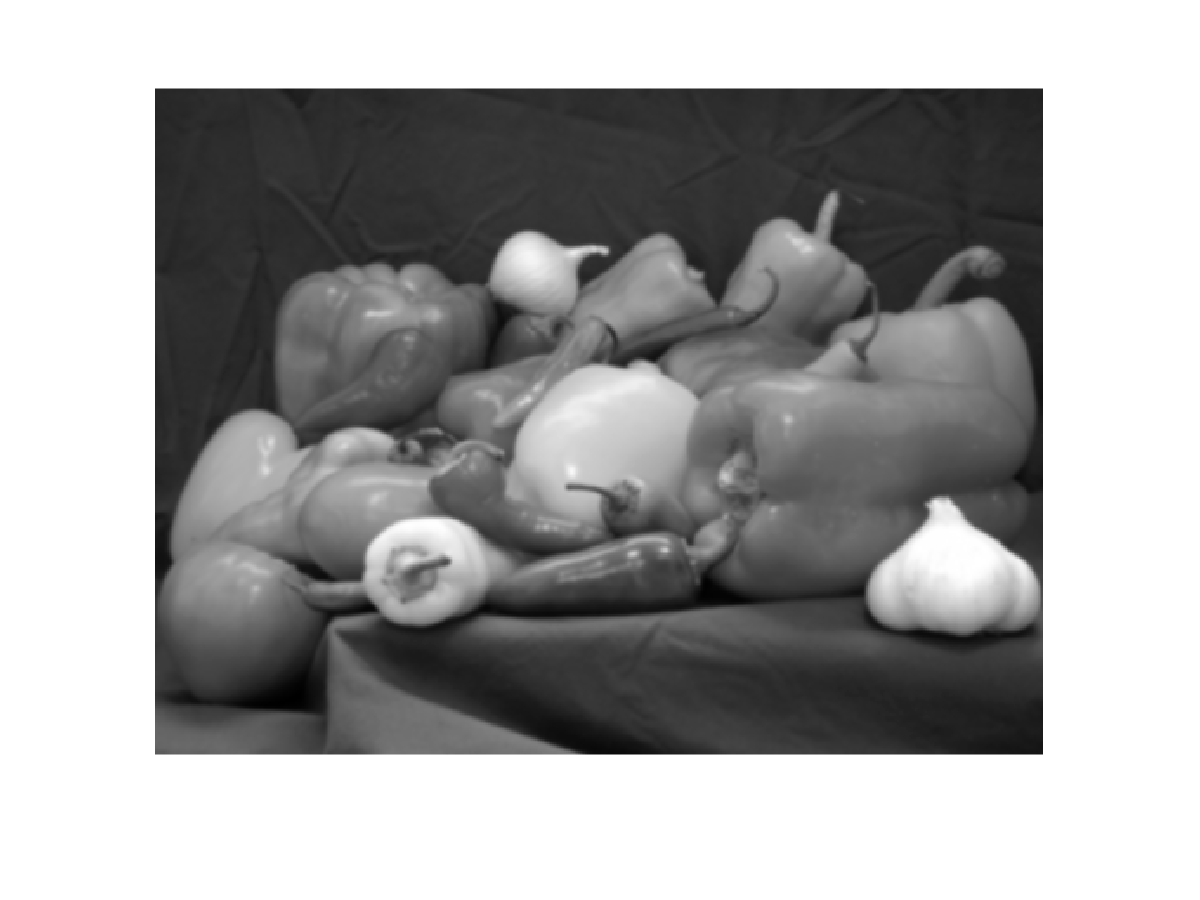
\includegraphics[scale=0.2]{images/peppersFB_c1}  &
		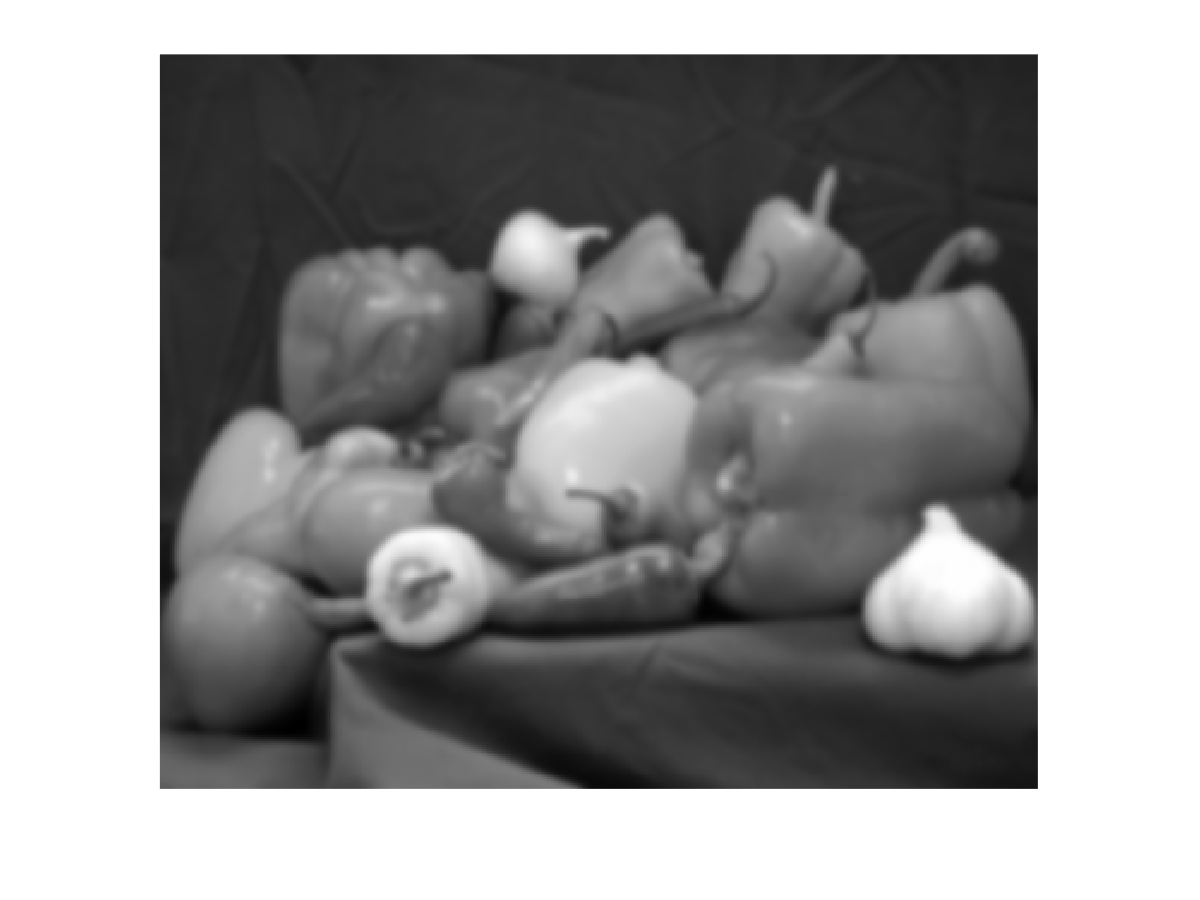
\includegraphics[scale=0.2]{images/peppersFB_c2}  &
		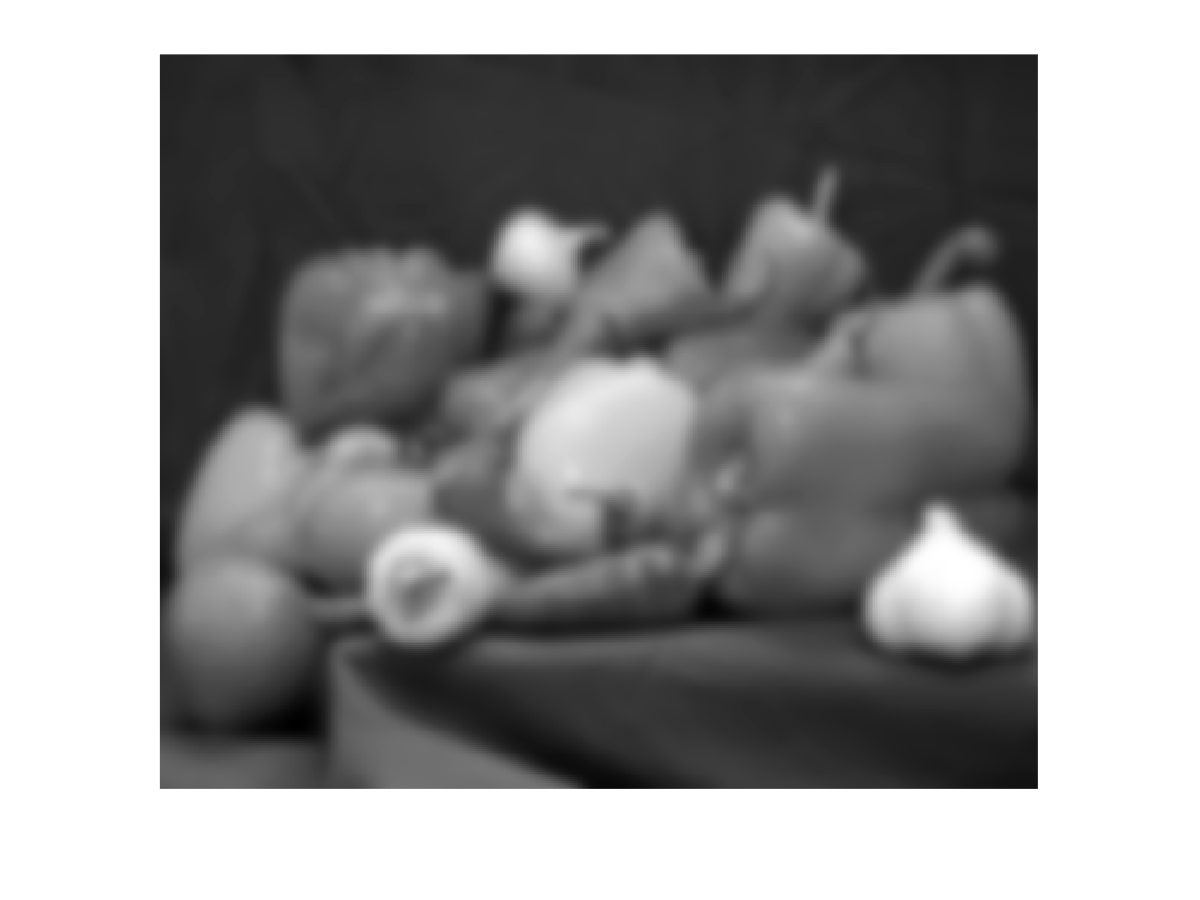
\includegraphics[scale=0.2]{images/peppersFB_c3}  \\
		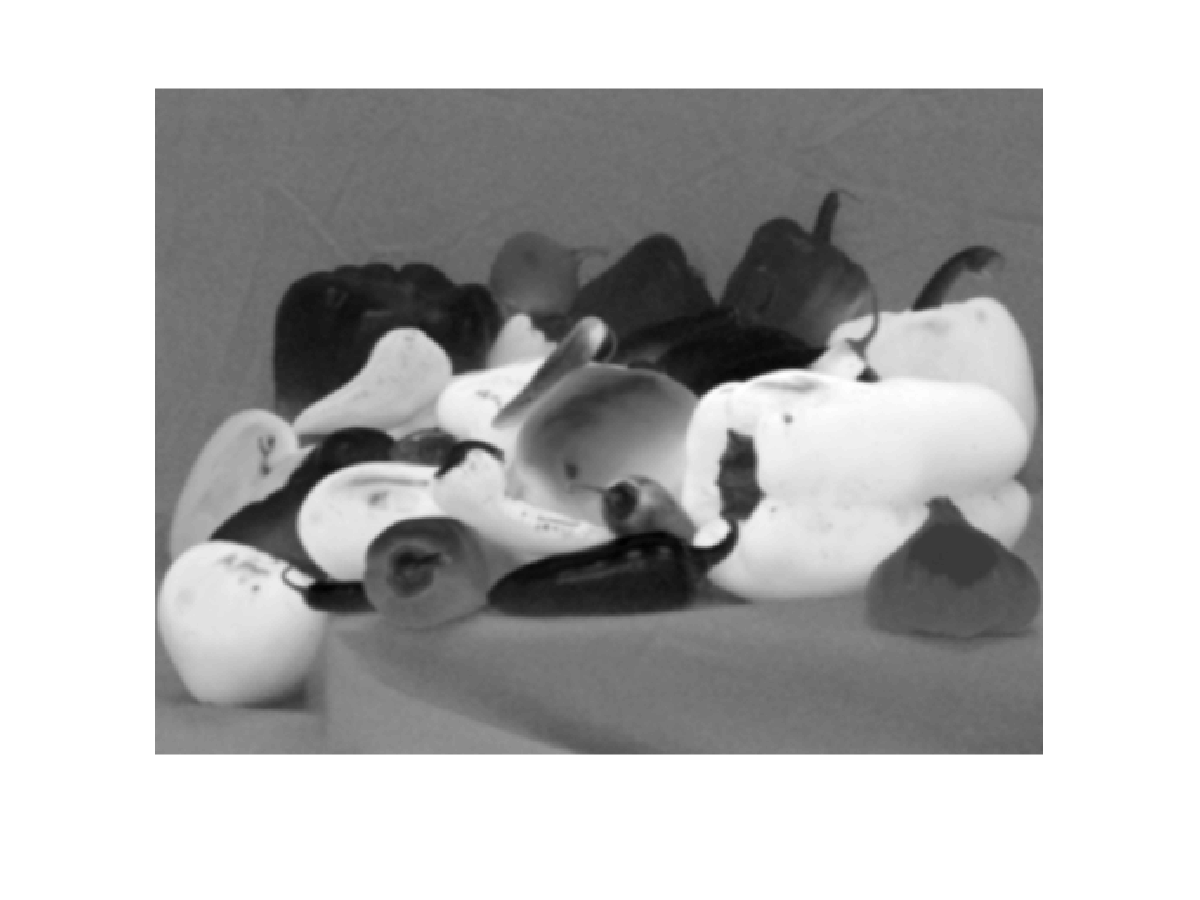
\includegraphics[scale=0.2]{images/peppersFB_c4}  &
		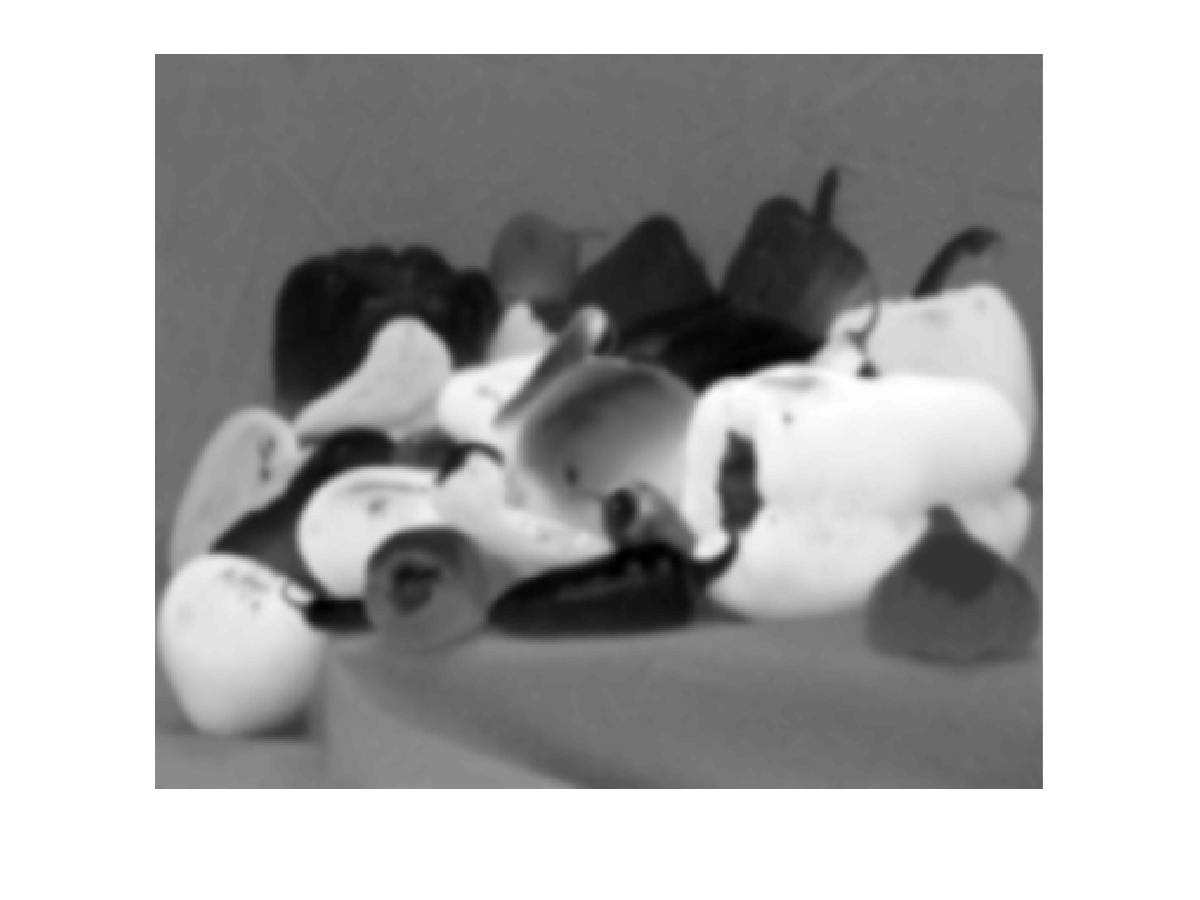
\includegraphics[scale=0.2]{images/peppersFB_c5}  &
		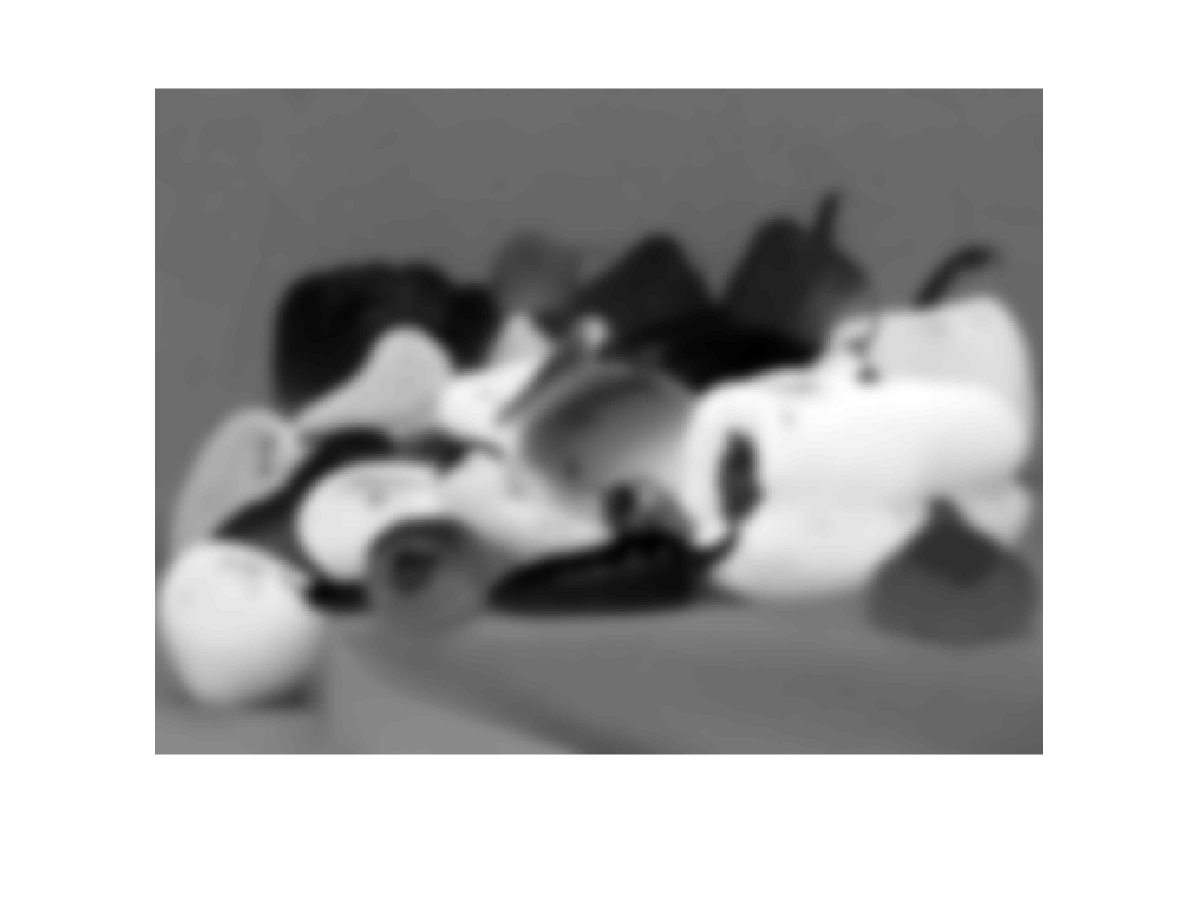
\includegraphics[scale=0.2]{images/peppersFB_c6}  \\ 
		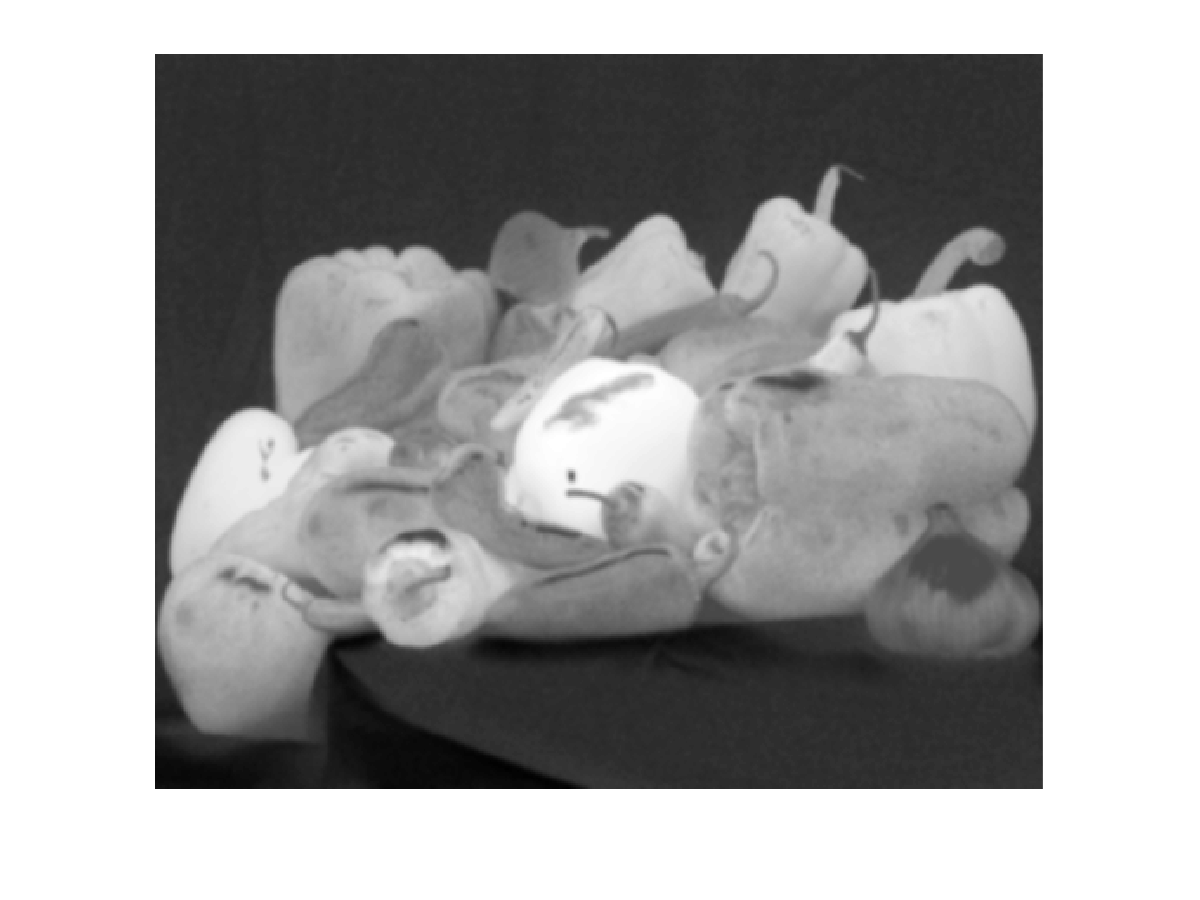
\includegraphics[scale=0.2]{images/peppersFB_c7}  &
		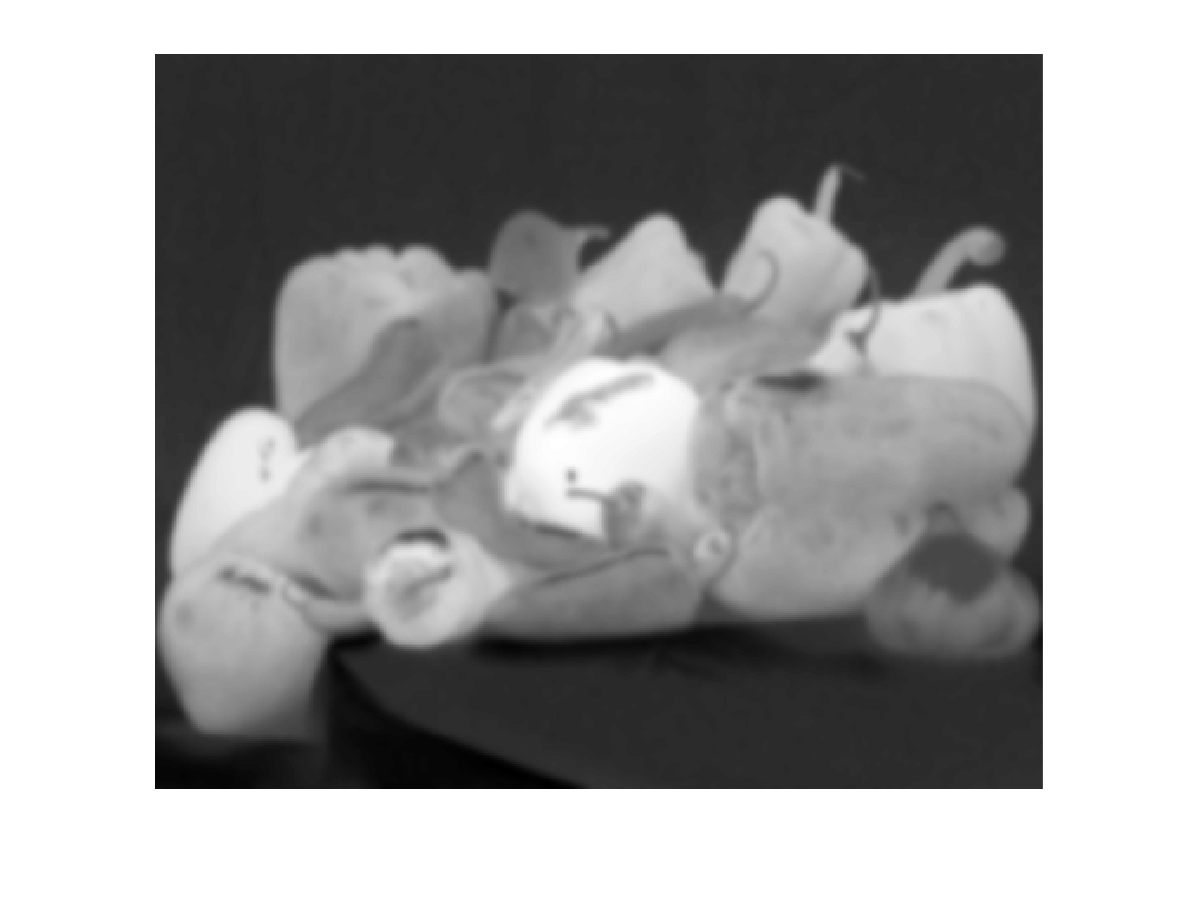
\includegraphics[scale=0.2]{images/peppersFB_c8}  &
		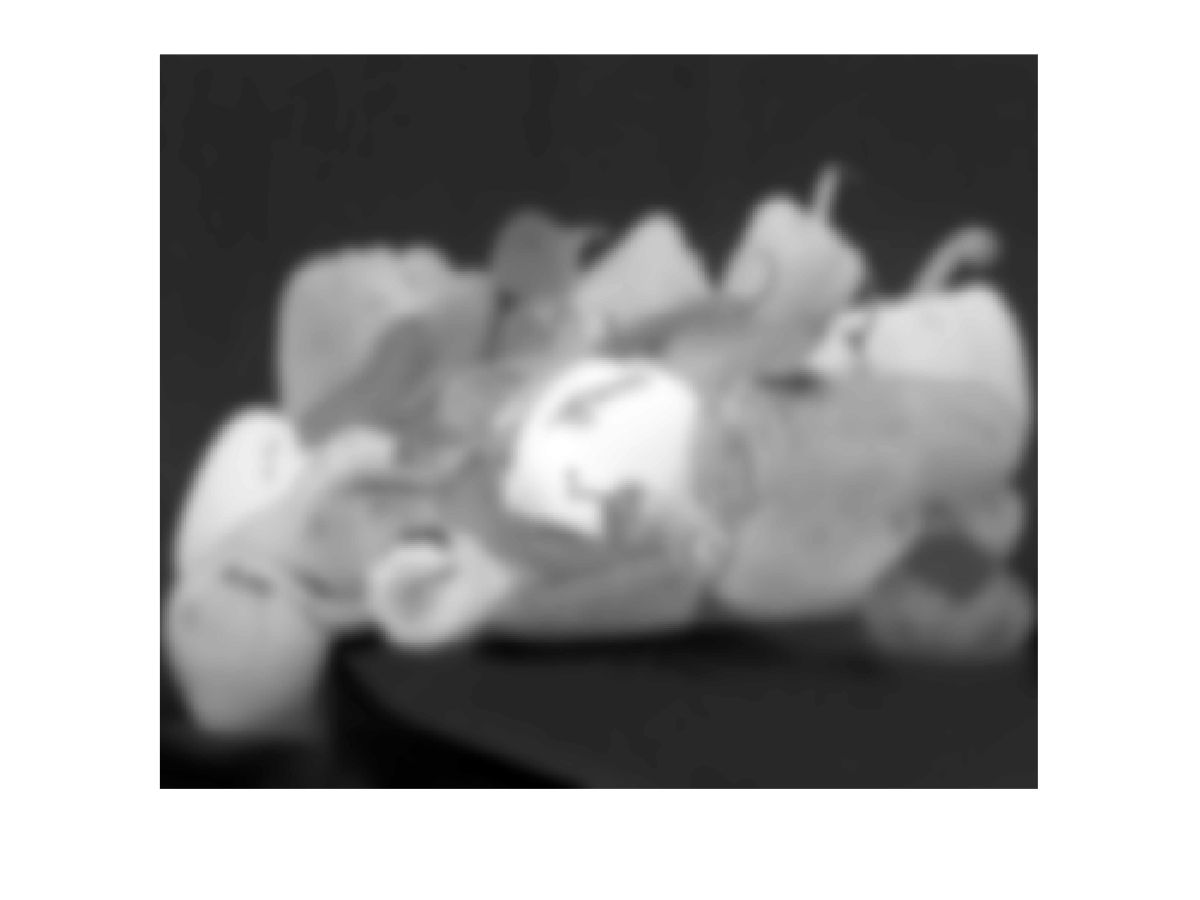
\includegraphics[scale=0.2]{images/peppersFB_c9}  \\
		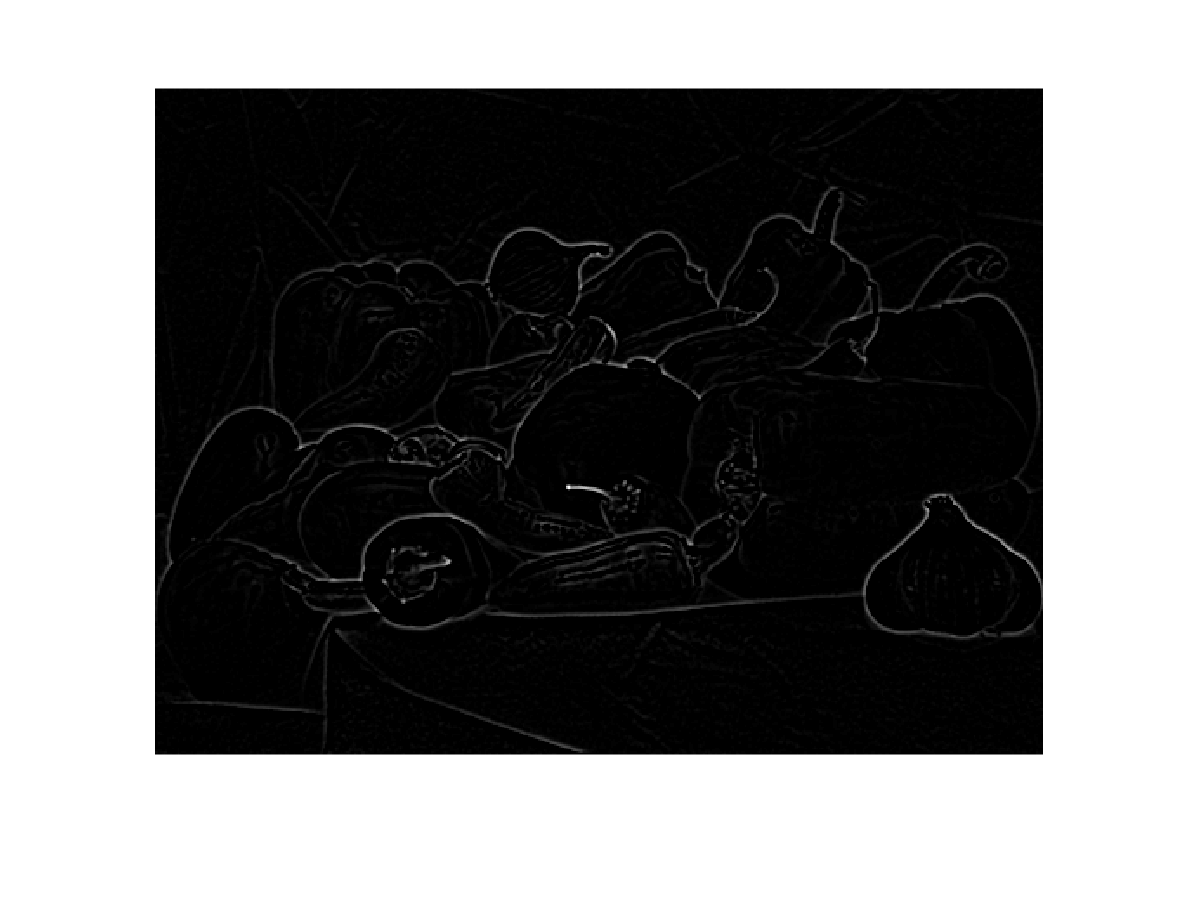
\includegraphics[scale=0.2]{images/peppersFB_c10}  &
		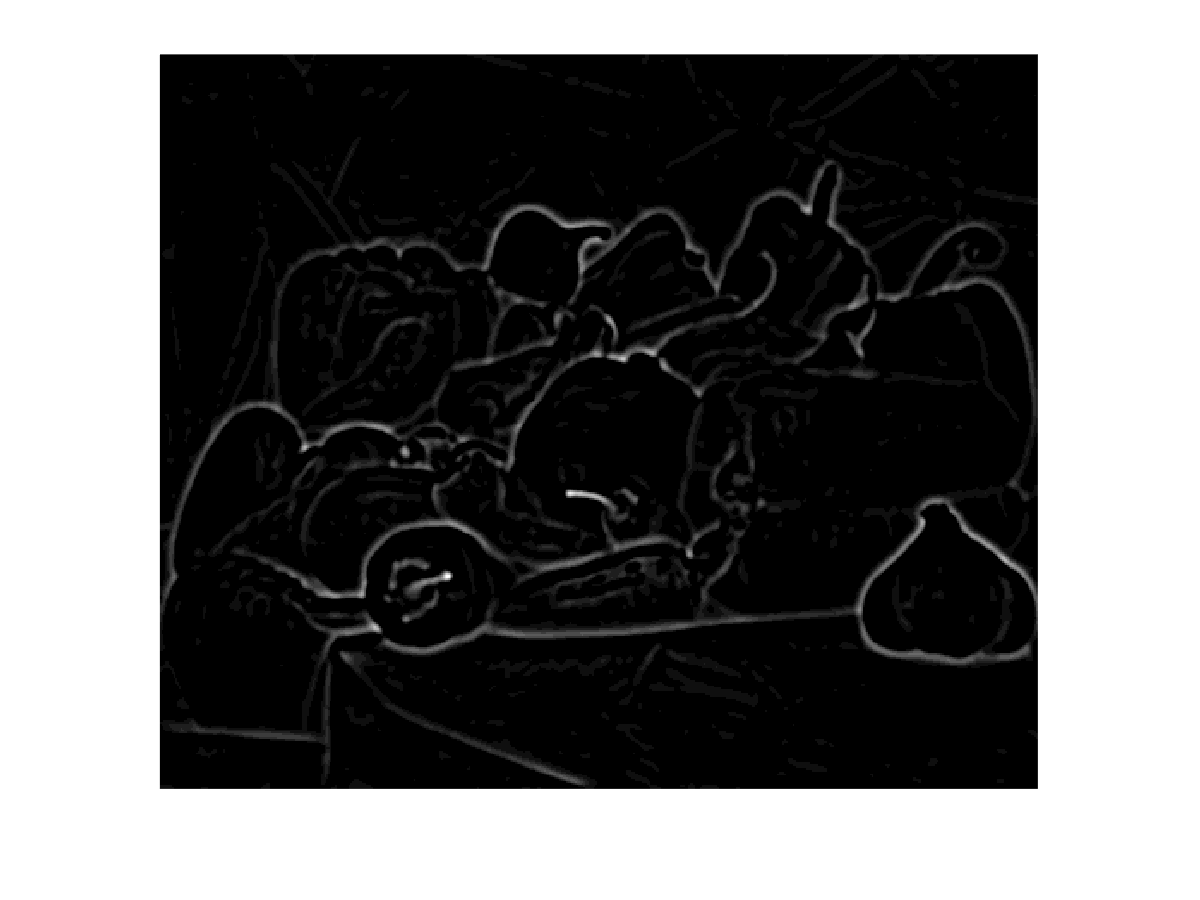
\includegraphics[scale=0.2]{images/peppersFB_c11}  &
		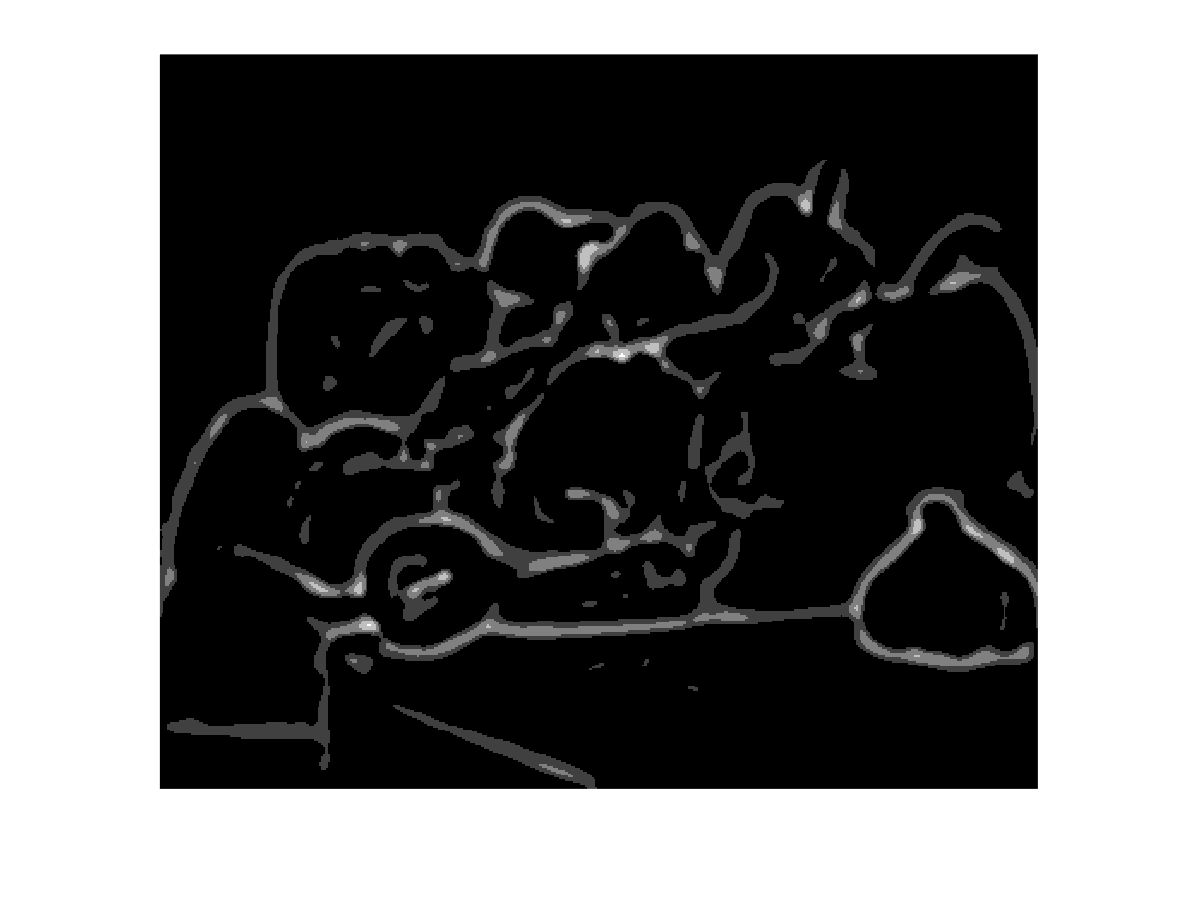
\includegraphics[scale=0.2]{images/peppersFB_c12}  \\
		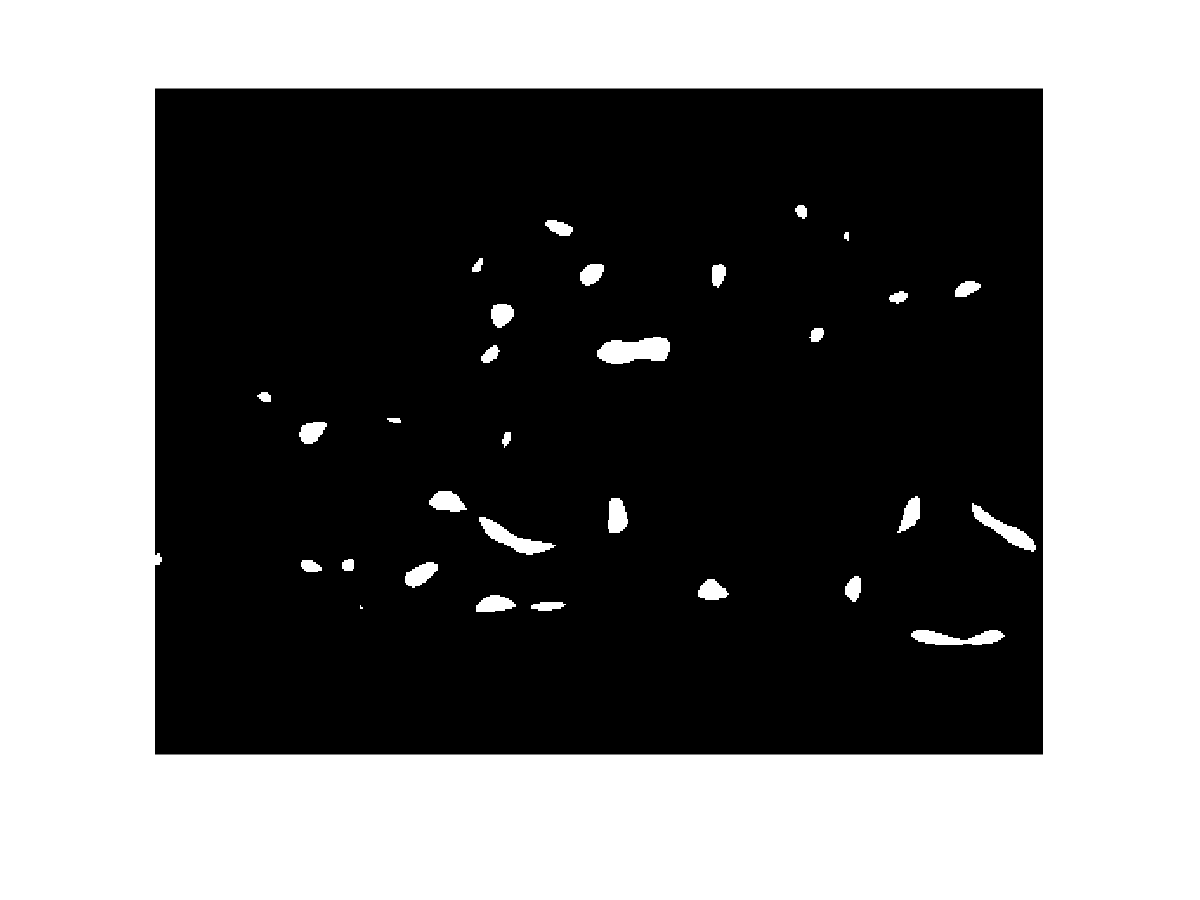
\includegraphics[scale=0.2]{images/peppersFB_c13}  &
		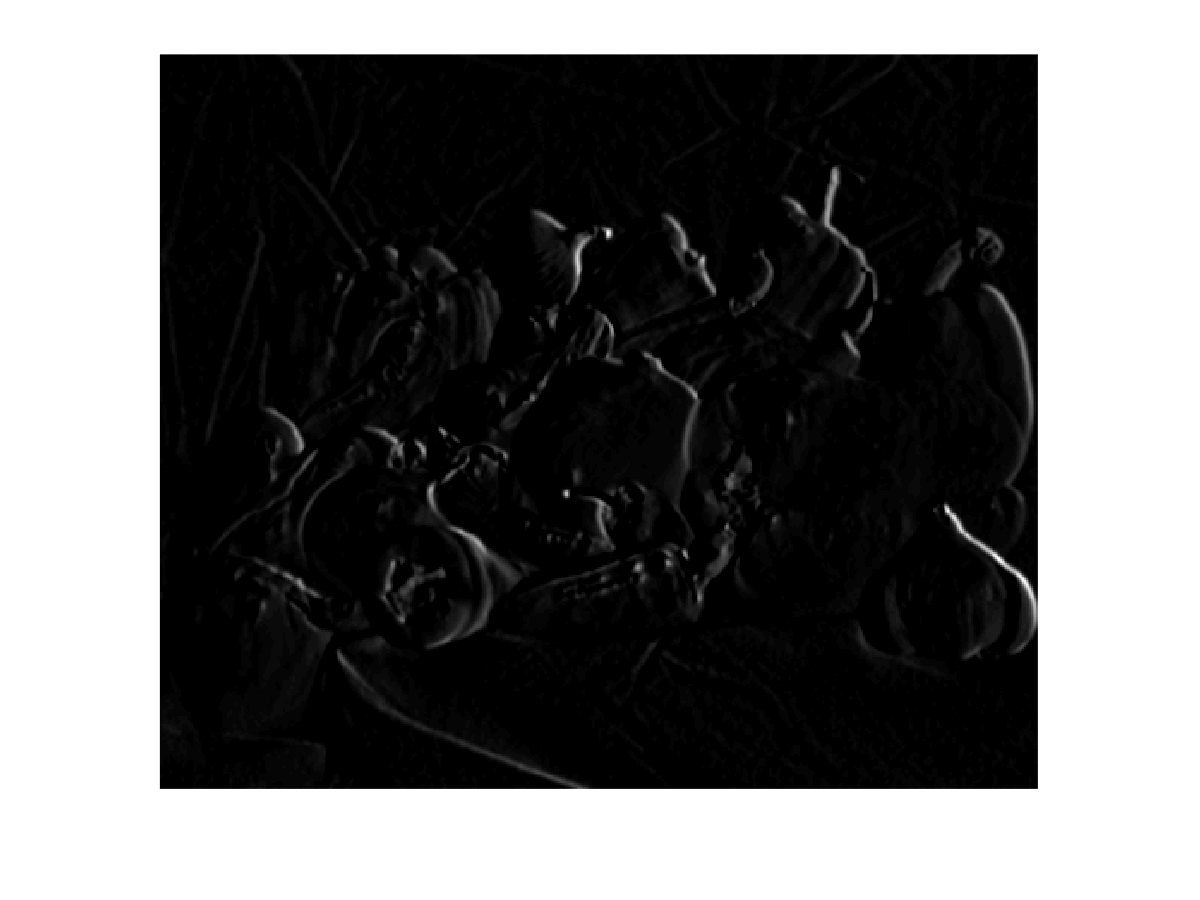
\includegraphics[scale=0.2]{images/peppersFB_c14}  &
		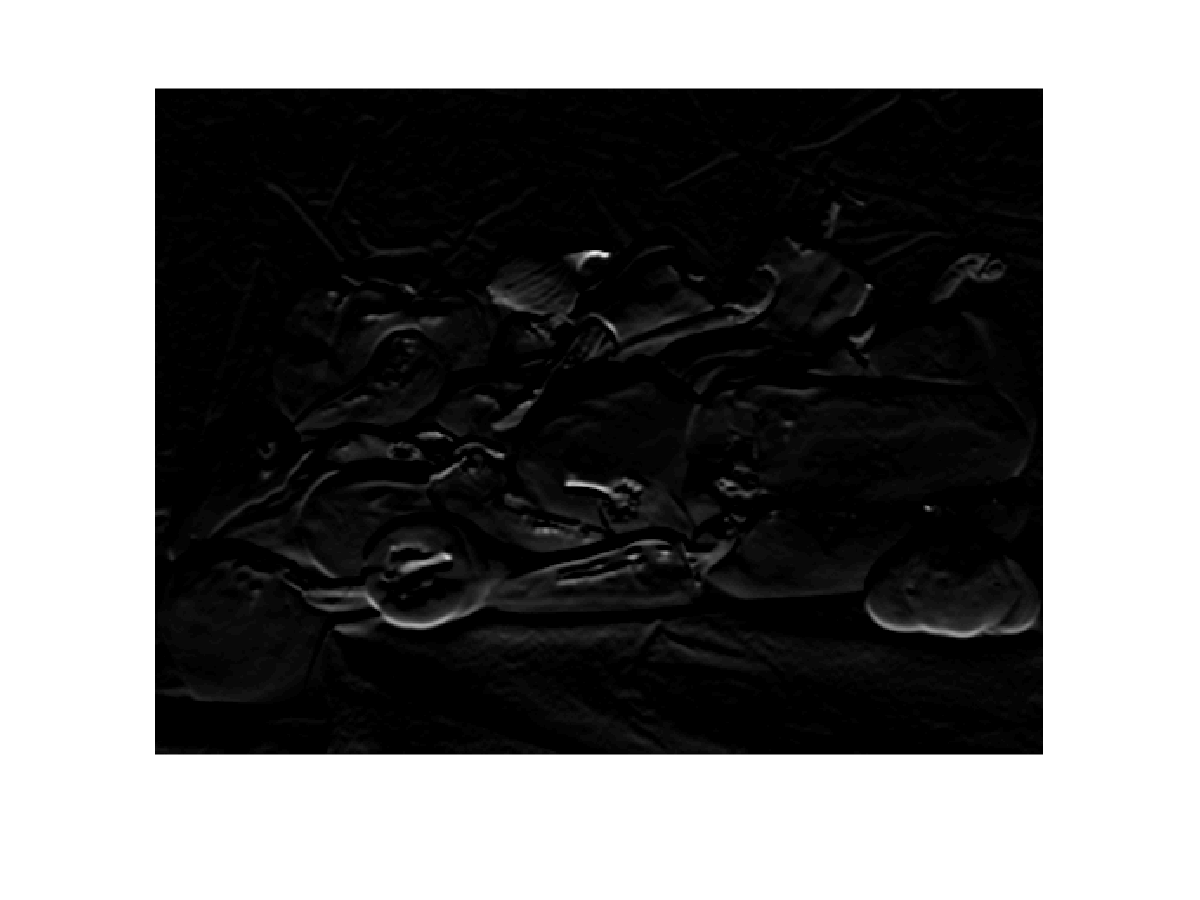
\includegraphics[scale=0.2]{images/peppersFB_c15}  \\
	\end{tabular}
	\begin{tabular}{cc}
		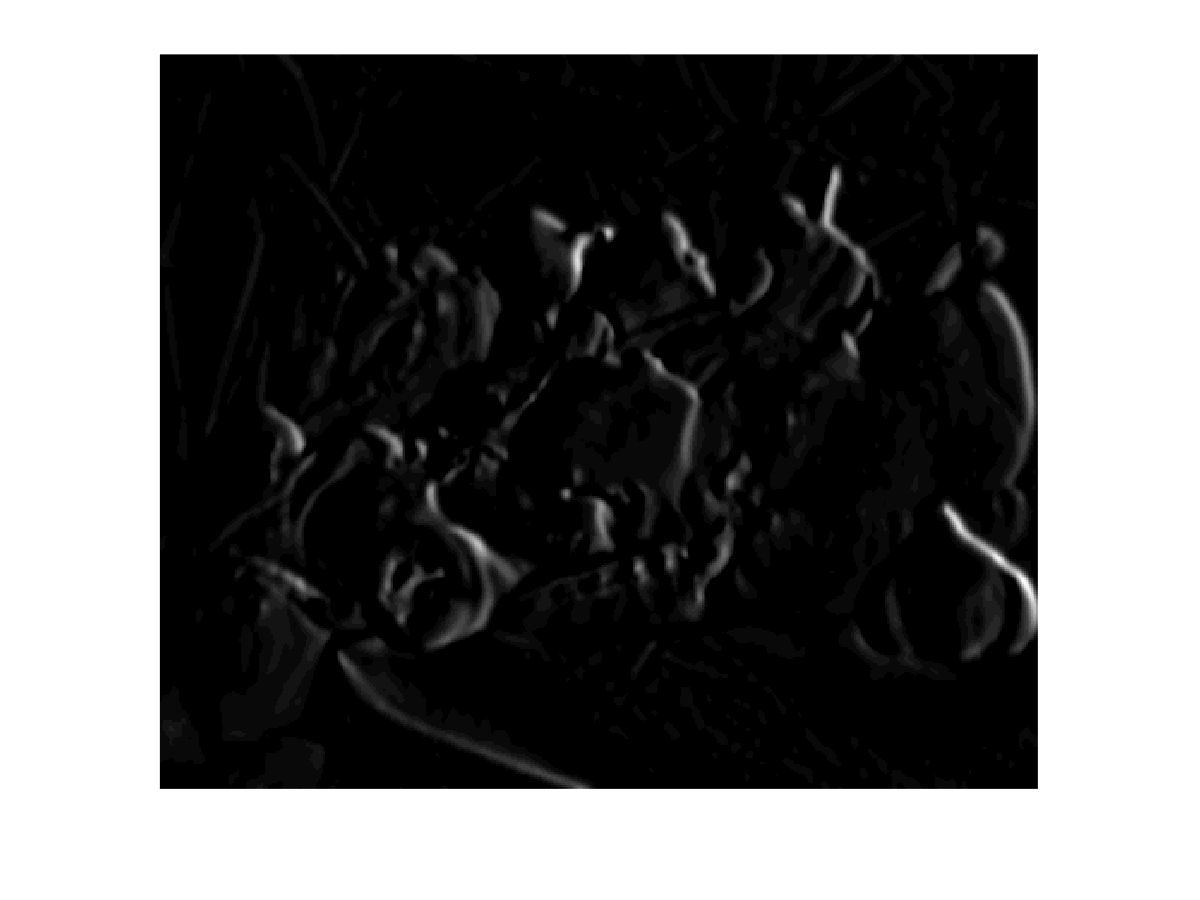
\includegraphics[scale=0.2]{images/peppersFB_c16}  &
		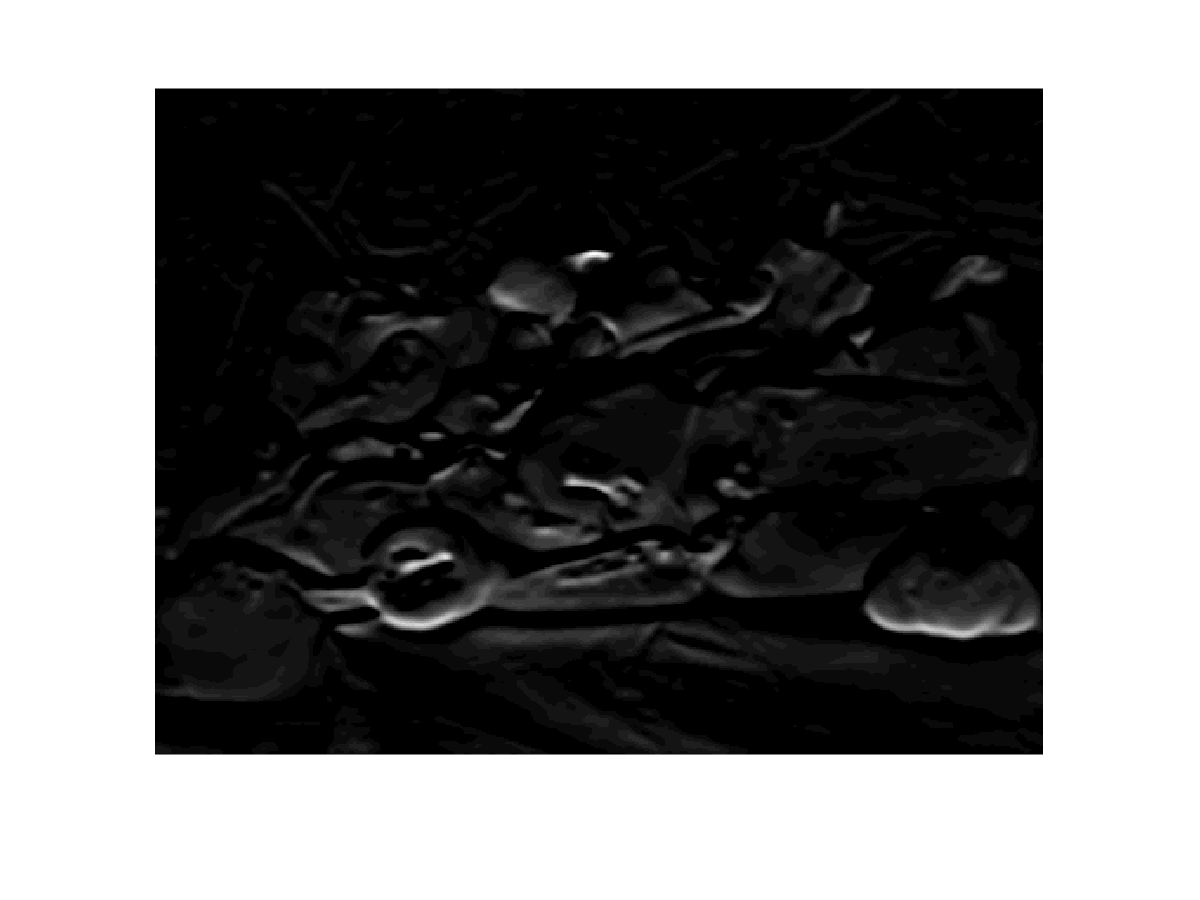
\includegraphics[scale=0.2]{images/peppersFB_c17}   \\
	\end{tabular}
	\caption{Applying the filterBank filters on the built-in ``peppers" image. Numbering of filters begins from top-left and proceeds in row-major order. Consult \texttt{filterBank.m} for details.}
	\label{fig:filterBankVis}
\end{figure}

\section{Results with initial set-up and minor modifications}
\label{sec:initSetup}

\subsection{SIFT features}
\label{sec:initSetupSIFT}

By ``initial setup", we refer to the set-up for \texttt{ps5} provided to us by the course instructors. This set-up concerns itself with a subset of the Caltech data featuring the class set \texttt{ \{pizza, platypus, pyramind, revolver, rhino\}}, a training ratio and dictionary building ratio of 0.5, 600 visual words generated for the dictionary, SIFT feature extraction and nearest-neighbor encoding. Figure \ref{fig:initSetupNoWeights} shows the confusion matrices attained for this set-up.

%%% Insert figure initSetupNoWeights...

\begin{figure}[H]
	\centering
	\begin{tabular}{cc}
		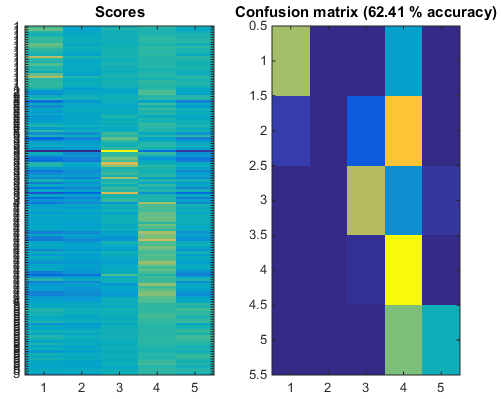
\includegraphics[width=.4\textwidth]{images/results/confMatInitSetupTrainNoWeights} &
		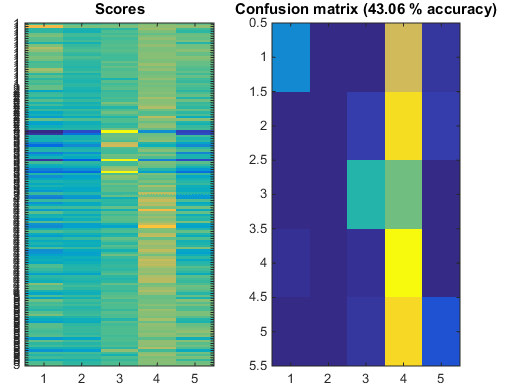
\includegraphics[width=.4\textwidth]{images/results/confMatInitSetupTestNoWeights} \\
	\end{tabular}
	\caption{Training and testing confusion matrices for the default problem set configuration.}
	\label{fig:initSetupNoWeights}
\end{figure}



With the aforementioned initial setup we had an overall training set accuracy of 62.41\%, whereas in the testing set we had 43.06\% accuracy. The exact per-class accuracies are shown in table \ref{tbl:initSetupResPerClass} Note that, ideally, since the train and test sets are extracted randomly with every run of the code, we should have presented the same experiment a number of times and taken the mean of the accuracies for both data splits, yet even those results in isolation provide for a good feel of what we can get with the default set-up.

We are already in position to present our first important optimization. We note that \liblinear\ performs One-Versus-All (OVA) classification. This means that, for $k$ classes, it trains $k$ binary SVM classifiers. Some (or all) of those $k$ binary classification problems might be imbalanced, because the positive data portions can be quite smaller than the negative data portions, or vice versa. By weighting the positive data portions by the number of negatives over the number of positives, we note a substantial improvement, shown in figure \ref{fig:initSetupWithWeights} and table \ref{tbl:initSetupResPerClass}. The reader may consult the function \texttt{trainSVM} to have an idea of how this is attained.

%%%% Insert figure initSetupWithWeights and the table initSetupResPerClass...

\begin{figure}[H]
	\centering
	\begin{tabular}{cc}
		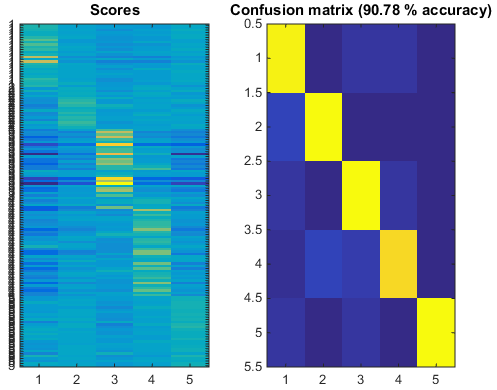
\includegraphics[width=.4\textwidth]{images/results/confMatInitSetupTrainWithWeights} &
		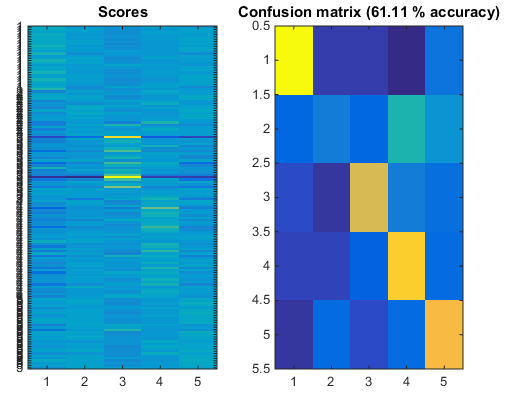
\includegraphics[width=.4\textwidth]{images/results/confMatInitSetupTestWithWeights} \\
	\end{tabular}
	\caption{Training and testing confusion matrices for the default problem set set-up with weighting of classes.}
	\label{fig:initSetupWithWeights}
\end{figure}

Furthermore, the course instructors mention in the write-up that when local encoding is used instead of nearest neighbor encoding, certain classes are expected to show better classification performance, in particular the class \texttt{rhino}. Table \ref{tbl:initSetupResPerClass} proves this claim, yet as can be seen in figure \ref{fig:initSetupWithLE}, local encoding does not necessarily lead to \textbf{overall} better classification performance for this initial set-up.

\begin{table}[H]
	\centering
	\begin{tabular}{c|c|c|c|c}
		\textbf{Class} & \textbf{No weights,} & \textbf{Weights,} & \textbf{No weights,} & \textbf{Weights,} \\ 
		 \multirow{2}{*}{\textbf{Name}} & \textbf{Nearest} & \textbf{Nearest} &  \textbf{Local} & \textbf{Local} \\
 		& \textbf{Neighbor} & \textbf{Neighbor} & \textbf{Encoding} & \textbf{Encoding} \\
		\cline{1-5} pizza  & 25.93\% & 81.48\%& 11.11\%& 29.63\%\\ 
		\cline{1-5} platypus & 0\% &  29.41\% & 17.65\%& 35.29\%\\
		\cline{1-5} pyramid & 48.83\% & 75.86\% & 65.52\%& 68.97\%\\
		\cline{1-5} revolver & 95.12\% &  75.61\% & 31.70\% & 31.71\%\\
		\cline{1-5} rhino & 10\% &66.67\%  &  \textbf{33.33\%}& 23.33\%\\
		\cline{1-5} Overall & 43.06\% & \textbf{69.44\%}& 33.33\% & \textbf{37.5\%}\\
	\end{tabular}
	\caption{Per-class and overall accuracies for the default set-up of the problem set with minor modifications. Note the improvement of results for class \texttt{rhino} when local encoding is used, as well as the overall improvement of the classification accuracy when we weight the classification problem (all those points of emphasis are \textbf{boldfaced}). The ``Overall" accuracy for the $3^{rd}$ column just happens to be the same as for the class \texttt{rhino} (33.33\%), i.e this is not a typo.}
	\label{tbl:initSetupResPerClass}
\end{table}

\begin{figure}[H]
	\centering
	\begin{tabular}{cc}
		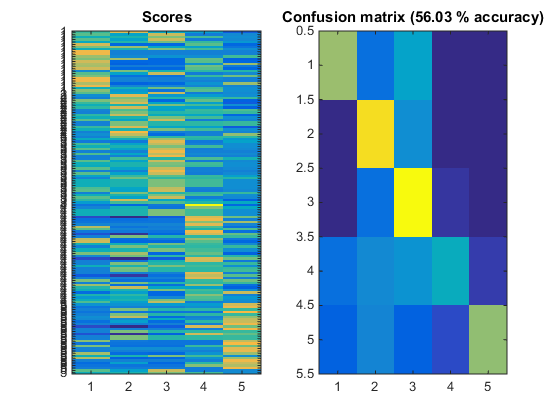
\includegraphics[scale=.4]{images/results/confMatInitSetupTrainWithWeightsLE} &
		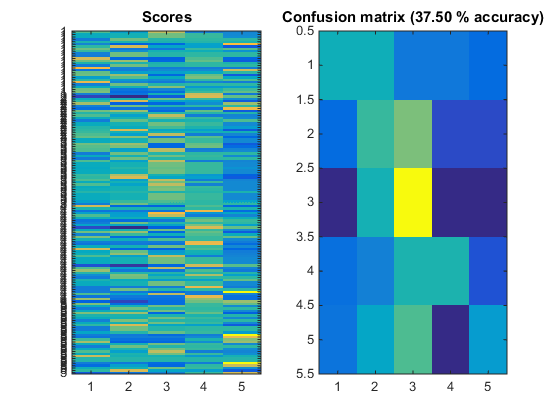
\includegraphics[scale=.4]{images/results/confMatInitSetupTestWithWeightsLE} \\
	\end{tabular}
	\caption{Training and testing confusion matrices for the default problem set configuration with weighting of classes and local instead of nearest neighbor encoding. Despite the fact that some classes can do better than others individually, the overall accuracy for this default set-up has dropped by approx. 30\% on the test set.}
	\label{fig:initSetupWithLE}
\end{figure}

\subsection{FilterBank features}

The filterBank features present a computational challenge at the dictionary learning stage. Specifically, since every $h \times w$ image ends up being represented by a vector of length $17 \times w \times h$, the computation of the squared two-norm between examples can become very costly and memory-intensive, particularly when \texttt{double}s are in play. If we feed the original data into the function \texttt{vl\_kmeans}, MATLAB eventually runs out of memory. In order to deal with this problem, we denote that, when compared to the number of 17-dimensional features involved in the learning of the clusters (which, for $k$ images of mean size $m\times n$, is $k \times m \times n$), the number of visual words to be learnt is small. For this reason, we make sure that we feed $K$-means a maximum of $10^4$ examples. More information is available in the comments of MATLAB function \texttt{getVocab}.

The confusion matrices of the original setup with filterBank features can be seen in figure \ref{fig:initSetupWithFB}. Note that since weighting positives has been deemed beneficial by previous results (see table \ref{tbl:initSetupResPerClass} for a refresher), we perform this optimization for all further experiments, including the one discussed here. Comparing figures \ref{fig:initSetupWithFB} and \ref{fig:initSetupWithWeights} we can see that FilterBank performs better when nearest neighbor encoding is used, while comparing figures \ref{fig:initSetupWithFB} and \ref{fig:initSetupWithLE} shows that it hurts a little in the case of local encoding.

\begin{figure}[H]
	\centering
	\begin{tabular}{cc}
		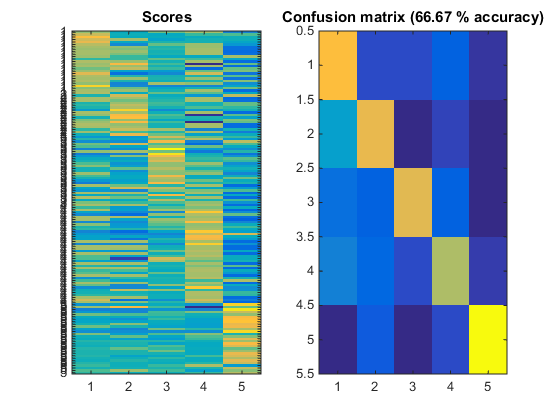
\includegraphics[scale=.4]{images/results/confMatInitSetupFilterBankLETrain} &
		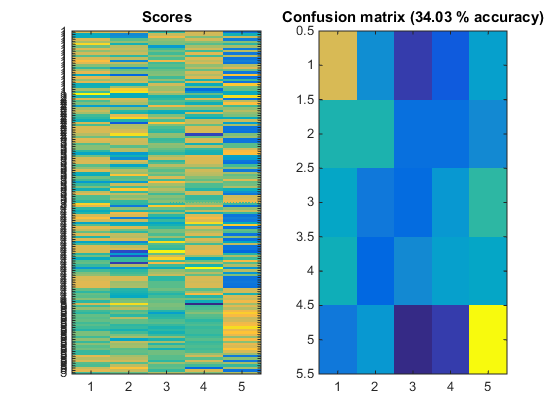
\includegraphics[scale=.4]{images/results/confMatInitSetupFilterBankLETest}
	\end{tabular}
	\caption{Confusion matrices for initial problem set configuration modified for extraction of FilterBank instead of SIFT features. Left: Testing accuracy when nearest neighbor encoding is used. Right: Testing accuracy when local encoding is used.}
	\label{fig:initSetupWithFB}
\end{figure}

\section{Results on entirety of Caltech dataset}
\label{sec:fullCaltech}

In this section, we analyze performance of BoVW classification across all 101 classes of Caltech. We extract SIFT features and vary the encoding type, as well as the various parameters (\texttt{dictRatioPerClass}, \texttt{numWords}, \texttt{TrainRatio}).The reason for not considering FilterBank is purely computational; the feature extraction method simply does not scale on the entire dataset, even when we used our aforementioned DeepThought allocation.  

\begin{figure}[H]
	\centering
	\begin{tabular}{ccc}
		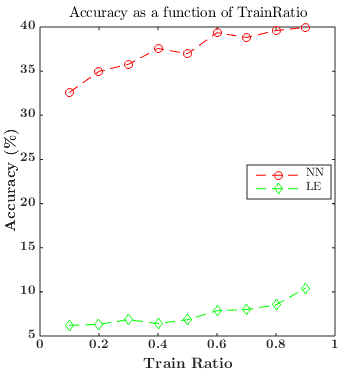
\includegraphics[scale=.4]{images/results/trainRatio.png} &
		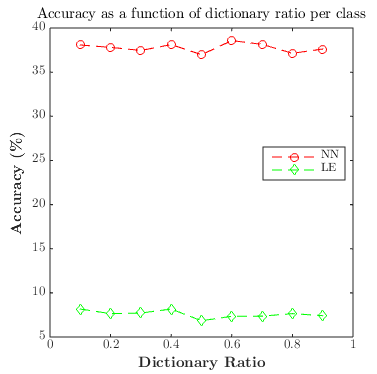
\includegraphics[scale=.4]{images/results/dictRatio.png} &
		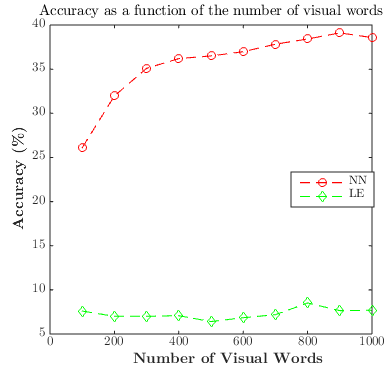
\includegraphics[scale=.4]{images/results/numWords.png} \\
		(a) & (b) & (c)
	\end{tabular}
	\caption{The effect of (a) \texttt{TrainRatio}, (b) \texttt{DictRatioPerClass} and (c) \texttt{numWords} on classification accuracy over the entire Caltech 101 dataset. To produce every plot, the other parameters were kept to their default values, e.g for (a) we kept \texttt{dictRatioPerClass} equal to 0.5 and \texttt{numWords} to 600. Best viewed in color.}
	\label{fig:fullCaltechGraphs}
\end{figure}


Figure \ref{fig:fullCaltechGraphs} shows the effect of tuning various parameters of the dataset. There are a couple of conclusions to be made after observing the figures:

\begin{itemize}
	\item Nearest neighbor encoding appears to globally outperform local encoding,  by a large margin of $\approx$30\%.
	\item Unsurprisingly, the learning algorithm tends to benefit from more training data over testing data. Care must be exerted, however, to avoid overfitting.
	\item It is not clear whether using a relatively large or small dictionary ratio parameter helps with classification accuracy.
	\item A larger number of visual words to build our vocabulary with leads to a more representative vocabulary and henceforth to increased classification accuracy.
\end{itemize}

All of those results are the product of jobs submitted to the DeepThought cluster. The full output of these jobs. in the form of .out files created by the SLURM scheduler, are available in the directory \texttt{sift\_results}, which we include in our submission.
\end{document}

